\chapter{\iflanguage{ngerman}{Übersicht Hybrider OP-Saal}{Overview}}
\label{sec:overview}

Weniger invasive Eingriffe, geringeres Risiko und kürzere Operations-und Krankenhausaufenthalte sind Anforderungen die heutzutage an Ärzte und Operationssäle gestellt werden \cite{DerDigitaleOperationssaal}. Anforderungen, welchen ein konventioneller OP-Saal nicht mehr gerecht werden kann, weshalb ein Umstieg zum Hybriden/ Digitalen/ Multifunktionalen oder auch Hochpräzisions OP-Saal statt findet. Egal welche der genannten Bezeichnungen verwendet wird, bei allen Variationen geht es darum den OP-Saal zu digitalisieren und Bildgebende Verfahren wie Röntgen oder Ultraschall während der Operation einzusetzen.

In den folgenden Kapiteln wird immer vom Hybriden OP-Saal die Rede sein und es werden die Unterschiede vom Hybriden zum Standard OP-Saal herausgearbeitet, sowie in welchen Einsatzgebieten der Hybride OP-Saal bereits verwendet wird und welche Vorteile dieser mit sich bringt.

\subsection{Hybrider OP-Saal vs. Konventioneller OP-Saal} 

\begin{figure} [H]
	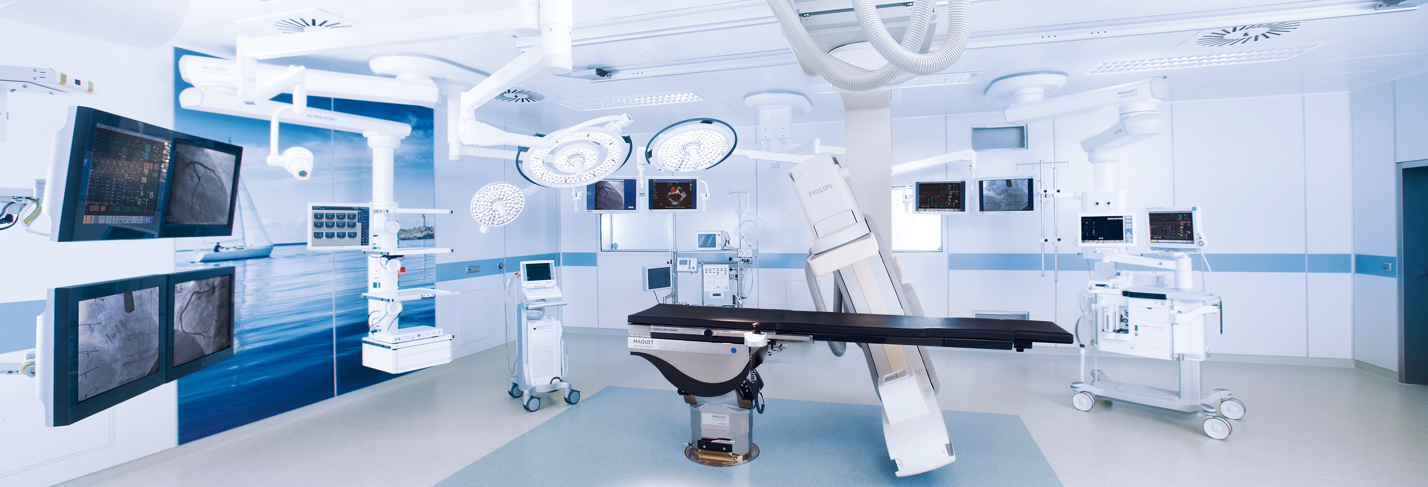
\includegraphics[scale = .3]{Content/Pictures/hybrid-or.png}
	\caption{Hybrider OP-Saal von Maquet. \cite{Maquet}}
	\label{fig:hybridor}
\end{figure}

Ein Hybrider OP-Saal (Beispiel in Abb. \ref{fig:hybridor}) ist die Verbindung aus einem sterilen konventionellen OP-Saal mit qualitativ hochwertiger Bildgebung, einem multifunktionalen OP-Tisch, einfacher Datenregistrierung und Dokumentation, ungehindertem Datenaustausch innerhalb und außerhalb des OPs und der Steuerung aller vorhandenen Geräte und Systeme über ein einzelnes Interface \cite{HybriderVsKonventioneller,KarlStorz}. Es wird nicht zwischen unterschiedlichen Abteilungen unterschieden, sondern ein Hybrider OP-Saal ist ein chirurgischer Arbeitsbereich, welcher fachbereichsübergreifend von der Neurochirurgie, Gefäßchirurgie, Onkologie, Kardiologie, Unfallchirurgie und vielen weiteren Bereichen genutzt werden kann \cite{Getinge}.\\
Mobile C-Bogen sowie Ultraschall- und Endoskopiegeräte trifft man in den meisten konventionellen Operationssälen an \cite{TechnicalConsiderations}, für komplexe Operationsvorgänge wie bspw. bei Transkathetertechniken und für die Visualisierung der dünnen Führungsdrähte, wird jedoch eine leistungsstärkere Ausrüstung benötigt. Die mobilen C-Bogen werden durch befestigte ersetzt und zur ergänzenden Ausrüstung des Hybriden OP-Saals können noch weitere Geräte für die intraoperative Bildgebung, wie Computertomographen (CT), Magnetresonanztomographen (MRT) oder Angiografieanlagen gehören \cite{OPderZukunft}. 
Die befestigten C-Bogen ermöglichen beispielsweise qualitativ hochwertige Echtzeitbildgebung mit Fluroskopie (Abb. \ref{fig:fluroscopy}) mit deren Hilfe Katheter durch den Körper geführt werden können, und Verfahren wie die Digitale Subtraktionsangiographie (Abb. \ref{fig:dsa}). Dabei werden zwei Bilder vom jeweilig abzubildenden Gebiet angefertigt, einmal mit und einmal ohne Kontrastmittel, und bei geschickter Subtraktion der beiden Bilder bleiben nur die Blutgefäße übrig \cite{CurrentAndFuture}. Darüber hinaus bieten MRT und CT die Möglichkeit hochauflösende Bilder von Geweben und Organen anzufertigen (Abb. \ref{fig:mrtct}).\\
Somit können während eines Operationsvorgangs Diagnose und Therapiekontrolle vorgenommen, sowie minimal invasive Behandlungsverfahren durchgeführt werden \cite{SHG-Kliniken}. Auch ist es möglich \glqq während der Operation - und nicht erst danach - Bildkontrollen durch[zu]führen und allenfalls Korrekturmaßnahmen [zu] ergreifen\grqq{} \cite{OPderZukunft}. 

\begin{figure}[!htb]
	\minipage{0.32\textwidth}
	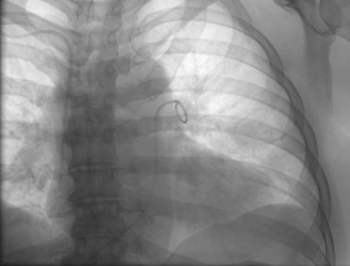
\includegraphics[width=\linewidth]{Content/Pictures/fluroscopy.png}
	\caption{Fluroskopie Aufnahme eines 2D Bildes mit einem C-Bogen \cite{CurrentAndFuture}.}
	\label{fig:fluroscopy}
	\endminipage\hfill
	\minipage{0.32\textwidth}
	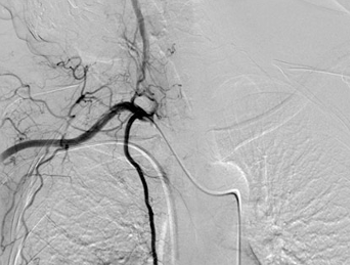
\includegraphics[width=\linewidth]{Content/Pictures/dsa.png}
	\caption{2D Bild mit Digitaler Subtraktionsangiographie (DSA) \cite{CurrentAndFuture}.}
	\label{fig:dsa}
	\endminipage\hfill
	\minipage{0.32\textwidth}%
	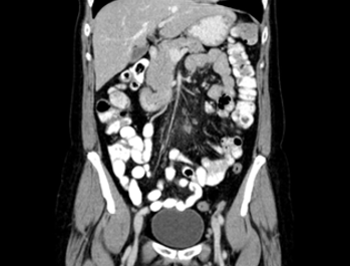
\includegraphics[width=\linewidth]{Content/Pictures/mrtct.png}
	\caption{CT-Aufnahme des Magens und Zwölffingerdarms \cite{CTBild}.}
	\label{fig:mrtct}
	\endminipage
\end{figure}

\subsection{Vorteile und wichtige Einsatzgebiete}

Wie Hybride OP-Säle Operationsvorgänge unterstützen, soll in der Neurochirurgie anhand der Kompensation des Brain Shifts, in der Gefäßchirurgie anhand des Setzens von Prothesen bei Aortenaneurysmen und in der Onkologie anhand der Tumorentfernung genauer erklärt werden.

\textbf{Neurochirurgie:}
Das Gehirn ist eine sehr komplexe dreidimensionale Struktur, bei der sogenannte Brain Shifts (Verschiebungen der Gehirnstruktur Abb. \ref{fig:brainshift}) während einer Operation auftreten können. Ursachen für Brain Shift können die Entfernung oder das Anschwellen von Gewebe, sowie der Verlust von Hirnwasser sein. 
Kommt es während einer Operation zu den oben genannten Verschiebungen, dann stimmen die vor einer Operation angefertigten CT oder MR Bilder der Gehirnstruktur nicht mehr mit der aktuellen Struktur überein. Bild geführte neurochirurgische Systeme (Image Guided Neurosurgical Systems, kurz IGNS), die normalerweise während der Operation als Navigationshilfe dienen, können dann nur noch begrenzt richtig arbeiten. Durch die inkorrekten Bilddaten entsteht ein größeres Risiko für den Patienten und die Operationsergebnisse werden verschlechtert.\\
Intraoperativer Ultraschall (iUS) oder intraoperative MR-Bilder (iMR) können diesem Problem entgegen wirken und die fehlenden Informationen ergänzen, sodass das IGNS wieder sinnvoll verwendbar ist.
Der Einsatz von iMR ermöglicht, während der Operation regelmäßig hochauflösende Bilder von der Gewebestruktur des Gehirns anzufertigen und im Falle eines Brain Shifts entsprechend zu reagieren. Auch bei anderen neurochirurgischen Anwendungen wie der Hirnbiopsie, Entfernung von Tumoren oder der Drainage von Zysten kann iMR von großem Vorteil sein.\\
Obwohl iMR als verlässlichste Option gilt um Bilder vom Gehirn anzufertigen und Brain Shifts zu erkennen, hat iUS den großen Vorteil sehr kostengünstig Echtzeitzeitbilder zu produzieren. Die Kombination aus einem präoperativen MR Bild und intraoperativen Ultraschall reicht aus, um Gewebeveränderungen zu registrieren und die Korrektheit des IGNSs zu beurteilen. Es wird mittlerweile eine Genauigkeit von ungefähr 1,36mm erreicht und im Gegensatz zu iMR, mit einer Bildaufnahmezeit von 15 Minuten, kann ein iUS Bild in 5 Minuten aufgenommen werden.
Aufgrund der vergleichend schlechten Bildqualität gegenüber iMR wird Ultraschall bisher nur sehr begrenzt in der Neurochirurgie verwendet. Neue Ansätze (siehe Kapitel 4.1) ermöglichen jedoch die Möglichkeit einer genaueren US Bildgebung für diesen Bereich \cite{BrainShiftInTumorResection}.

\textbf{Gefäßchirurgie:}
Die Gefäßchirurgie profitiert von Hybriden OP-Sälen, da die intraoperative Echtzeitbildgebung erlaubt, den Fortschritt eines Katheters durch die Gefäße zu beobachten. Dadurch können das Ergebnis, wie das Setzen und richtige Sitzen einer Prothese, beurteilt werden.\\
In Bezug auf ein Aortenaneurysma, also eine krankhafte Erweiterung der Hauptschlagader, ergeben sich neue Möglichkeiten der Operationsdurchführung. Da diese Aneurysmen ruptieren und zu lebensbedrohlichen Blutungen führen können, muss ab einem gewissen Durchmesser der Erweiterung eine Prothese gesetzt werden. Die Operation kann entweder als offene Operation mit konventionellen Prothesen durchgeführt werden oder mit einem schonenden Verfahren und Implantation großer maßgefertigter Gefäßprothesen im Hybrid OP-Saal (siehe Abb. \ref{fig:bauchaorten}). \\
Die offene Operation, bei der bei Bauchaneurysmen ein großer Schnitt in die Bauchdecke gemacht werden muss, weist zwar gute Langzeitergebnisse auf, ist aber sehr belastet und mit langen Erholungszeiten verbunden. Da Aortenaneurysmen verstärkt im höheren Alter, also über 60 Lebensjahre, kommt für viele Patienten eine offene Operation nicht mehr in Frage. \\
Beim schonenden Verfahren wird vor der Operation ein CT Bild angefertigt, welches dann mit den während der Operation entstehenden zwei- oder dreidimensionalen Bildern der Röntgenkontrolle zusammengeführt wird. Dies ermöglicht, eine Stent-Prothese minimalinvasiv einzusetzen. Mithilfe eines Katheters kann dabei über einen kleinen Zugang in der Leiste durch das abgebildete Gefäß navigiert werden. Eine zusätzliche Software zur Navigationshilfe trägt dazu bei, die Prothese sicher und schnell durch die Gefäße ans Ziel zu bringen \cite{Aortenaneurysma,DresdnerUniklinikum,TickendeBombeImBauch}.

\textbf{Onkologie:}
In der Onkologie hat man im Hybriden OP-Saal den Vorteil, dass nachdem ein Tumor entfernt und bevor die Operation abgeschlossen wurde, ein Kernspin mit dem MRT gemacht werden kann ohne den Patienten transportieren zu müssen. So kann man sicherstellen, dass tatsächlich keine Rückstände des Tumors übersehen wurden bzw. sollte dem nicht der Fall sein, dann kann direkt Nachkorrigiert werden. Durch diese Korrekturmöglichkeit können manche Folgeoperationen dem Patienten erspart bleiben \cite{AerzteZeitung}.\\
Die Zweckmäßigkeit des intraoperativen MRT wurde damit bestätigt, dass in mehr als einem drittel der Fälle, in denen eine vollständige Entfernung des Tumors angenommen wurde, Rückstände festgestellt und somit nachkorrigiert werden musste \cite{BrainShiftInTumorResection}.

\textbf{Fazit:} Zusammenfassen lässt sich sagen, dass Hybride OP-Säle präziseres, sicheres und schonenderes operieren durch minimalinvasive Eingriffe ermöglichen, welche weniger belastend für den Patienten sind und kleinere Narben hinterlassen \cite{DresdnerUniklinikum}. Das wiederum  führt zu kürzeren Krankenhausaufenthalten und zu Kosteneinsparungen in der Nachbetreuung und -behandlung. \\
Der beliebig positionierbare OP-Tisch, zusammen mit dem hochbeweglichen C-Bogen  ermöglichen optimale Röntgenbildaufnahmen, die zur Unterstützung vor, während und nach der Operation eingesetzt werden können \cite{DresdnerUniklinikum}. Entscheidungen über den Fortlauf der Operation können so besser getroffen werden, Ergebnisse beurteilt und gegebenenfalls nachkorrigiert werden.

\begin{figure}[!htb]
	\minipage{0.45\textwidth}
	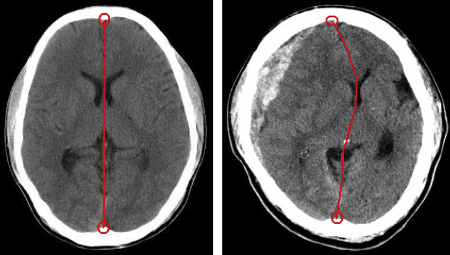
\includegraphics[width=\linewidth]{Content/Pictures/brainshift.png}
	\caption{Verschiebung der Mittellinie des Gehirns (midline brain shift) durch Anschwellen von Gewebe \cite{BrainShiftImage}.}
	\label{fig:brainshift}
	\endminipage\hfill
	\minipage{0.45\textwidth}%
	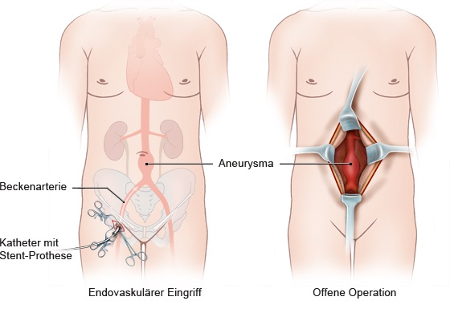
\includegraphics[width=\linewidth]{Content/Pictures/bauchaorten.png}
	\caption{(links) Endovaskulärer Eingriff bei einem Bauchaortenaneurysma mit Stent-Prothese im Hybriden OP-Saal gegenüber (rechts) einer offenen Operation mit normalen Prothesen im Konventionellen OP-Saal \cite{BauaortenaneurysmaBild}.}
	\label{fig:bauchaorten}
	\endminipage
\end{figure}